%	@file FinalDocumentation.tex
%	@author Thomas Bogue, Joseph Ciurej
%	@date Spring 2014
%	
%   LaTeX source file for the design document for the CS411 project.  More 
%   information about the requirements for this documentation file can be found
%   here: "https://wiki.cites.illinois.edu/wiki/display/cs411sp14/Final+Report+Instructions"

\documentclass{article}
\usepackage[parfill]{parskip}		% Package that improves paragraph formatting
\usepackage[pdftex]{graphicx}		% Package that faciliates figure insertion
\usepackage{float}					% Package that allows for arbitrary figure insertion
\usepackage{hyperref}				% Package that allows for text hyperlinking
\usepackage{tikz}					% Package that facilitates box rendering

% The following code block changes a few parameters of the page to make the
% text fill up more space on any given page.  For our liking, the default 'article'
% template is too sparse.
\addtolength{\voffset}{-2cm}
\addtolength{\textheight}{4cm}
\addtolength{\oddsidemargin}{-1.5cm}
\addtolength{\textwidth}{2cm}

% This command creates blue boxes around class names.
% @see "http://tex.stackexchange.com/questions/36401/drawing-boxes-around-words"
\newcommand\appname[1][]{\tikz[overlay]\node[fill=green!20,inner sep=2pt, anchor=text, rectangle, rounded corners=1mm,#1] { DatBigCuke };\phantom{ DatBigCuke}}
\newcommand\gcalendar[1][]{\href{https://www.google.com/calendar}{Google Calendar} }
\newcommand\gravatar[1][]{\href{http://en.gravatar.com/}{Gravatar} }

\newcommand{\insertdiagram}[2]
{
	\begin{figure}[H]
		\centering
		\fbox{\includegraphics[height=#2]{figures/#1}}
		\caption{UML Diagram for the #1 Class}
	\end{figure}
}

\begin{document}

	% Title Page %
	\title{DatBigCuke: Final Project Report}
	\author{Eunsoo Roh, Joshua Halstead, Kyle Nusbaum, Thomas Bogue, Joseph Ciurej \\
		University of Illinois: Urbana-Champaign (CS411)}
	\date{\today}
	\maketitle

	% Table of Contents %
	\tableofcontents
	\clearpage

	% Body %
	\section[Project Overview]{Brief Project Overview}
	The primary purpose of this project was to create an online service for college
	students to help them manage their academic deadlines.  Our primary hope
	is that the application can serve a centralized repository for college
	students' deadlines and aid them in organizing these deadlines in a 
	straightforward and digestable manner.  
	
	The application is meant to be used by many students in college courses to 
	facilitate the crowdsourcing of deadline times for course homeworks and other 
	various assignments.  Additionally, the application provides functionality to allow 
	student groups to organize group meetings to work towards completing their related deadlines.

		\subsection[Motiviation]{Project Motivation}
		The main motivation for creating this service was a common need among
		the group members for a centralized deadline management system.  We all
		found that the highly variate means by which courses and college groups
		distribute deadlines made effective deadline management a near impossibility.
		In creating the \appname web service, we aim to eliminate this problem by 
		allowing users to congregate and collaborate on deadline data entry.  
		
		Additionally, we've found that organizing group meetings with the purpose of 
		working towards completing deadlines is an equally difficult task with the
		large variability in group member schedules.  The need to efficiently find
		potential times for such meetings was another primary motivator for the
		features we implemented in the \appname service.

		\subsection[Affordances]{Project Affordances}
		The \appname service has the capacity to help users accomplish a number of
		tasks, including more efficient deadline management, more effective
		group scheduling, and more centralized group organization.
		
		Users can sign up for groups in \appname and enter deadlines associated 
		with these groups. Once enough users of a group have entered a deadline
		for a particular assignment, the official time for this deadline is
		determined by aggregating these user-entered deadlines using statisical
		analysis methods.

		The integration of autocomplete makes the process of signing up for
		academic groups seamless.  After seamlessly signing up for their
		courses through the \appname interface, users can begin to create their
		own user subgroups and begin scheduling meetings to accomplish the
		tasks associated with their deadlines.  
		
		The means of finding appropriate scheduling times is made painless 
		through integration with \gcalendar, which the application pulls scheduling 
		data from to determine the availability times of each group member.  
		The \appname service uses each users selected \gcalendar calendars in
		addition to a few other user input values (e.g. off limits times, deadline 
		for the meeting, et cetera) in order to determine optimal meeting times.  
		Also, through the use of asynchronous email handlers, the \appname service 
		allows users to quickly and easily propogate calculated meeting times, 
		making the process of scheduling even easier.


	\section[Functions and Features]{Project Functions and Features}
	In order to more fully describe the affordances of the \appname application,
	we'll now flesh out all the functions and features of the service in more
	detail.  Specifically, we'll detail the primary features of the application 
	in brief, then move to overview a few of the basic functions provided by the 
	application before finally highlighting the two key features of the application
	(i.e. deadline aggregation and group meeting scheduling with \gcalendar).

		\subsection[Feature List]{Concise Functions and Features List}
		\begin{itemize}
			\item Users can sign up for the service by providing their email 
			address and credentials.  Each user must verify their email address 
			before being allowed to utilize the service.

			\item Authenticated users may view and edit their personal information 
			on their profile page (including the \gravatar icons associated with their
			sign-in email).

			\item Users can link their account to \gcalendar from their main
			profile page by filling out the linked Google service verification form.

			\item Authenticated users can view and modify the hierarchy of academic
			groups that they're signed up for on the groups page.

			\item Users can add courses through the root group page (i.e. the
			user institution group page) with user entry assisted by autocomplete.
			Users can also add private subgroups to courses through one of the groups page.

			\item Users can add additional members to private subgroups with
			user email entry assisted by autocomplete.

			\item Users can freely leave groups that aren't dependent on their
			presence.

			\item Users can add deadlines for assignments associated with groups
			through the group interface with assignment name entry assisted by
			autocomplete.

			\item Once enough users have added a deadline for an assignment,
			these deadlines are aggregated using statistical analysis methods
			and broadcast to all users (and listed as community-driven deadlines).

			\item Users can request the scheduling of a group meeting for a
			particular deadline through the group interface.  This interface 
			allows the user to customize the meeting duration, off-limits
			times, and the required attendees.  A list of good meeting times
			will be returned based on this information and user \gcalendar data.
			
			\item Given a list of potential meeting times, the users are
			provided an interface that allows them to choose a good meeting
			time and to broadcast this time with a custom message to all group
			members.
		\end{itemize}

		\subsection[Basic Functions]{Overview of A Few Basic Functions}
		For our function to describe, we chose a nice piece involved in adding
		a member to a private group. That is, the auto-completion of the email
		of potential users to be added. After the user types the first two
		characters of an email, we offer auto-completions of members who
		are able to be a part of this private group. We send the characters
		through ajax to a request handler on the back-end, which then forms
		a SQL query that looks like this:

			\begin{verbatim}
			SELECT u.id, u.email, gm.group_id
			FROM user AS u
			JOIN group_membership AS gm
			ON u.id = gm.member_id
			WHERE gm.group_id="CS 411" AND u.email LIKE "jh%"
			\end{verbatim}

		(in this example the parent group to the private group the user is 
		adding to would be ``CS 411'', and the user is trying to look up the
		email ``jhalstead@gmail.com''.) The database would then return a list of
		potential emails, say it gives back [``jhalstead@gmail.com'',
		``jhalla@gmail.com'']. This gets passed back to the front-end, and JQuery
		populates a dropdown menu with these two emails. Of course after the
		user chooses one and hits Submit, the email is inserted appropriately
		into the database.


		\subsection[Advanced Functions]{Overview of Advanced Features}
		Our first advanced feature is what we call the deadline aggregation. The idea
		behind the aggregation is that many people in a class will add canonical deadlines
		such as the times a homework is due, or the time of an exam. It would be nice,
		then, if these deadlines were pushed to all the other users in that class.
		That is the goal of the aggregation algorithm. We implement by having
		three levels of ``trust'' for a deadline. The lowest level is a Personal
		deadline, the next level is a Communal deadline (one that many people have 
		agreed on,) and an Endorsed deadline (one that is confirmed by a group leader
		or professor.) The different levels are given different colors on the site.

		The aggregation algorithm fits into this scheme by automatically deciding
		on, and creating, the Communal deadlines. We use statistical analysis methods
		to determine if a deadline should be made Communal, given all the entered
		Personal deadlines, and taking into account the size of the group. Once a deadline
		has been aggregated, all users in the course (even if they add the course after
		the aggregation,) will be able to view this deadline.

		Our second feature is the group meeting scheduling. The meeting scheduler
		allows a private group to find a time to work together on a deadline by
		giving a list of times when everyone that needs to make the meeting is free,
		and allowing the user to choose from these times and send an email to each
		group member informing of the meeting. This turned out to be very challenging,
		involving many different components of the project. The availability of each
		group member is based on their Google Calendars, so we had to work with the
		Google API to get this information. Users our asked to give our app read
		access to their Google Calendars, and this access is stored with the user.

		The scheduling itself uses an algorithm we wrote to determine times where
		everyone is free, taking into account the meeting duration, everyone's
		available times, and overnight ``off-limits times'' the user chooses (so
		that meetings are not scheduled for silly times like three in the morning.)
		The available times are used to populate a modal, the user can choose one
		and give an email message, and we craft and send the email to all the group
		members in the meeting.


	\section[Project Implementation]{Project Implementation and Design}

        \subsection[Database Design]{Database Design\footnote{The full schema
        for our database is located in the appendix of this document.}}

        The primary design assumptions that \appname operates under and which
        influenced the database design are listed below.

        \begin{itemize}\itemsep0em
            \item There must be only one ``official group'' per course / section.
            \item A group can have subgroups or users as members.
            \item A course can have multiple sections, but not vice versa.
            \item An appointment has exactly one organizer (user).
            \item An appointment can have multiple users as attendees, and a
                user can attend multiple appointment.
            \item Deadlines can have multiple entities (user/group) and entities
                can have multiple deadlines.
            \item A group can have zero or more deadline authorities, and a user
                can be deadline authority of multiple groups.
        \end{itemize}

        The primary tables of \appname, viewable in Figure~\ref{fig:er},
        are the \texttt{group}, \texttt{user}, \texttt{group\_membership}, and
        the \texttt{deadline}/\texttt{metadata} tables. Central to the design of
        \appname was the idea of a \texttt{Group}, which represents both courses
        (i.e.\ public groups) and private subgroups. A group has many attributes,
        including a maintainer who serves as the group's authority (e.g.\ the
        professor of a course or the team leader of a group project). 

        By design, groups and their members form a tree-like heirarchy which is
        rooted by an institution (e.g UIUC). The nodes of the heirarchy can be
        one of two things: a subgroup or a user. For example, CS 411 is a group
        in our tree and contains a set of students and a set of project groups.
        This abstraction reduces duplication and offeres a cleaner interface to
        design around.

        Given that \appname is a deadline management web service, it is natural
        that the \texttt{Deadline} and \texttt{DeadlineMetadata} tables are
        central to its operation. Deadlines consist of a time, a name, and a type.
        From a user's perspective, they never interact with or directly view an
        entry from the \texttt{Deadline} table.
        
        Instead, we use a layer of indirection to allow user's to have independent
        control over their deadlines. This creates our ability to aggregate
        common deadlines into a canonical deadline. This layer of indirection is
        introduced via the \texttt{DeadlineMetadata} table, which consists of a
        \texttt{user\_id}/\texttt{deadline\_i}d pair and a reference to additional
        metadata (e.g.\ notes). It is the metadata that user's see and manipulate.
        Given this indirection, we're free to identify common deadlines amongst
        a group and generate a canonical deadline--called a \textit{communal}
        deadline--that is propogated to all current and future members of the
        group. Moreover, if a maintainer creates a similar deadline as an existing
        \textit{communal} deadline or a set of users' personal deadline, we
        upgrade and consolidate the matching deadlines to an \textit{endorsed}
        deadline. This new deadline is also propogated throughout the group and
        replaces the deadlines of all the original matching deadlines. Note that
        personal metadata is always preserved during aggregation and endorsement. 

        \begin{figure}[h]
            \centering
            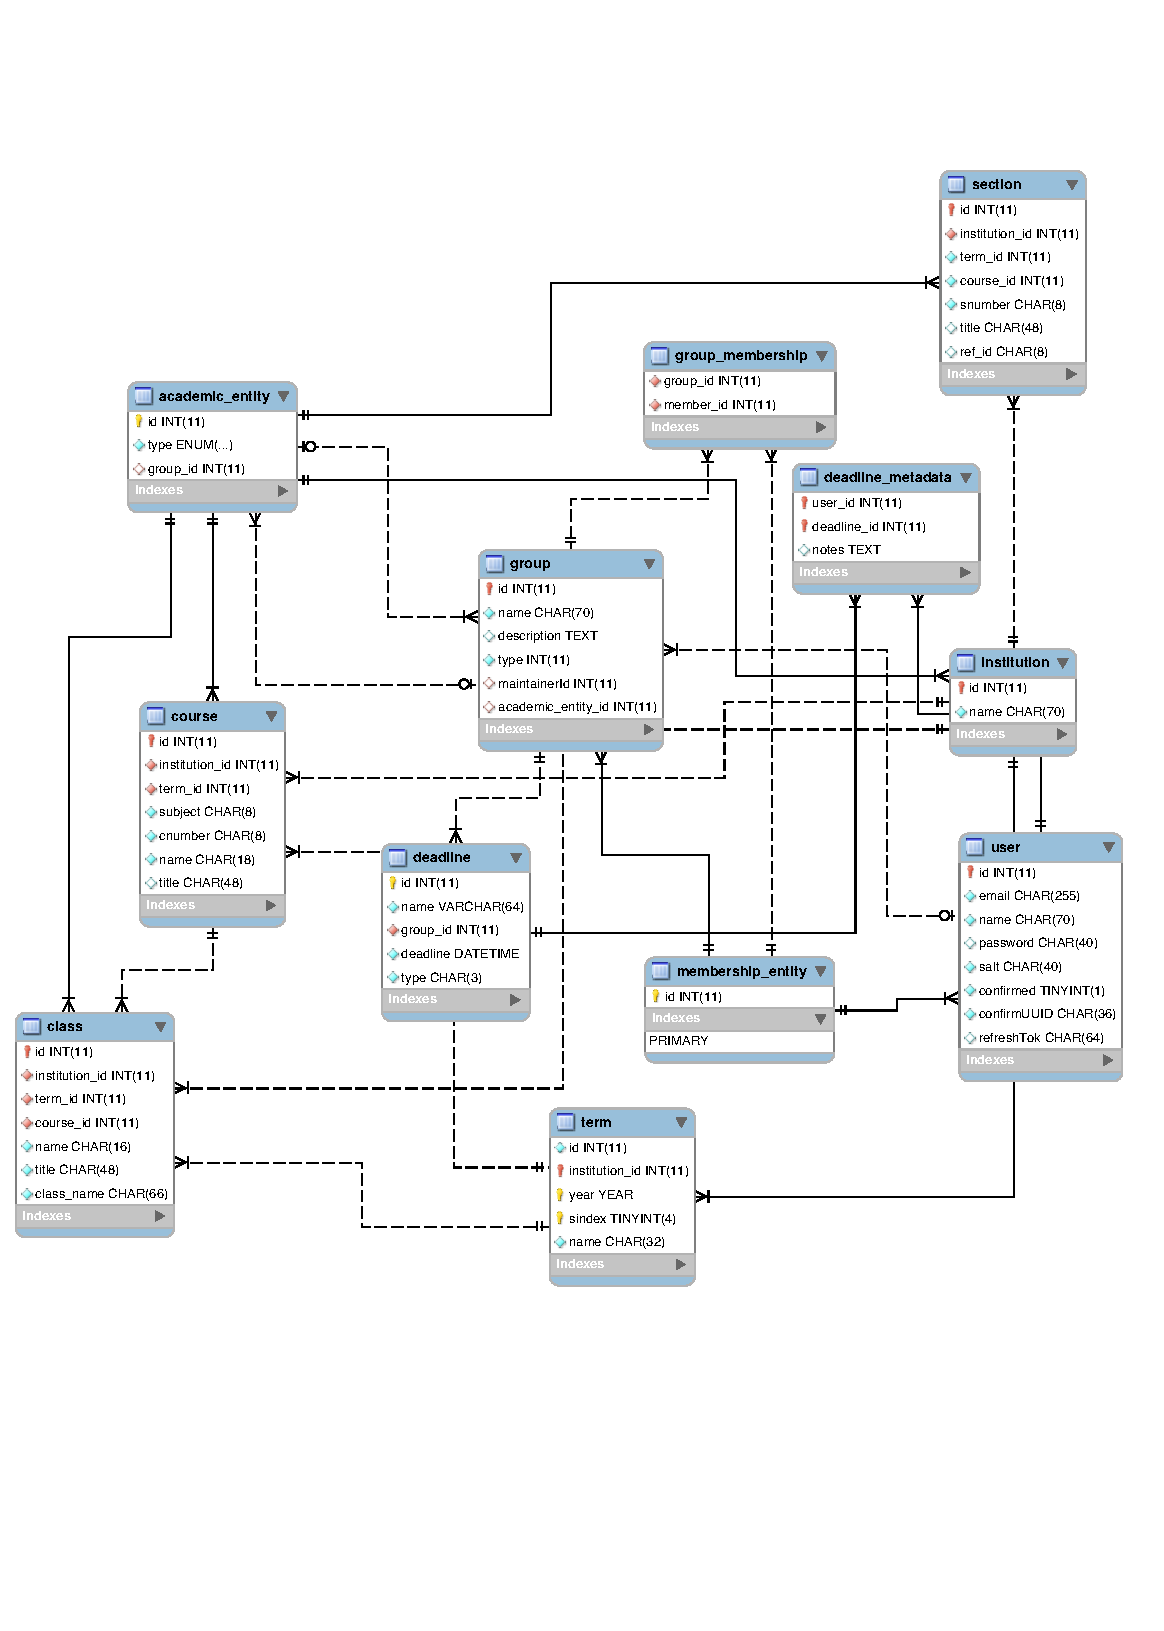
\includegraphics[width=1\textwidth]{figures/er-diagram.pdf}
            \caption{\appname entity-relationship diagram using Information 
            Engineering notation.}
            \label{fig:er}
        \end{figure}

        \subsection[Data Gather]{Data Gathering}
        The major data needed to be collected and processed was course
        information, which we discovered were available via the
		\href{http://courses.illinois.edu/cisdocs/explorer}{CIS Data Explorer App}.
        The CIS Data Explorer App provides access to course information in the
        form of XML. Its structured like a tree or forest where the root(s) are
        the schedules in XML for all the available years. Predictably, their
        children represent the semesters for that particular year. This tree-like
        structure continues until the leaves (i.e. the individual sections of a
        course) are reached.

        As such, we wrote a Python script to crawl and parse the tree of XML pages
        and then insert the processed data into our tables. After processing courses and
        sections for each semester, the script executes a SQL query to
        generate the entities of smallest unit, which we call a ``class''. This
        unit was strategically designed to split courses by their section titles,
        as some courses deserved some distinction between different sections e.g.
        CS 498 Algorithms vs. CS 498 Cloud Computing. The design of the crawler
        is general and performant enough so as to be adaptable to other university's
        schedules with minor tweaks.

		\subsection[Implementation Schedule]{Project Implementation Schedule and Tasks}
        The core of the \appname web service consists of a front-end,
        user-facing interface, a set of page request handlers for each individual
        web page, a set of request handlers for asynchronous \texttt{POST}s and
        \texttt{GET}s that allow seamless user interaction with \appname, a
        database abstraction layer, and the \texttt{MySQL} database itself.
            
            \subsubsection[Task Delegation]{Delegation of Project Tasks}
             Like many web services, our \appname web service lent itself well
             to the classic front-end, back-end, middleware division of labor.
             The back-end team consisted of Kyle and Eunsoo. Joe handled the
             front-end, and Tom and Josh the middleware. Naturally, some overlap
             occurred throughout the development of \appname, but we generally
             stayed true to the outlined division of labor. Below is the basic
             task delegation:

            \begin{itemize}\itemsep0em
                \item Eunsoo
                    \begin{itemize}\itemsep0em
                    \item Database creation, schema design, and server
                        maintainence.
                    \item Development of the database abstraction layer. This
                        is code that allows us to interact with the database
                        without directly constructing SQL queries everywhere.
                    \end{itemize}

                \item Kyle
                    \begin{itemize}\itemsep0em
                    \item Also worked on the database abstraction layer and the
                        request handlers.
                    \item Wrote user email verification and scheduler email
                        sending.
                    \end{itemize}

                \item Josh
                    \begin{itemize}\itemsep0em
                    \item Scraping course data from the UIUC course catalog.
                    \item Major work on the asynchronous request handlers which
                        bridge the front end to the back end.
                    \end{itemize}

                \item Tom
                    \begin{itemize}\itemsep0em
                    \item Wrote scheduling and aggregation algorithms.
                    \item Google API authentication and integration.
                    \end{itemize}
 
                \item Joe
                    \begin{itemize}\itemsep0em
                    \item Designed and created the website's front-end pages.
                    \item Also worked on the request handlers.
                    \end{itemize}

           \end{itemize}

			\subsubsection[Technical Challenges]{Technical Challenges}
			Working with the Google API was very difficult.
			Looking at the documentation, it seemed like it should have been more simple
			than it turned out to be. The main stumbling point was that Google refuses to
			send back data to anything other than an authenticated app, which can only be
			that one running on the actually server. Thus, testing any of the Google API
			usage locally was an impossibility. Since there were quite a few instances
			where the server was down during development, testing the Google API integration
			was often not something that could even be done. Unfortunately, the specifics
			of the Google authentication also turned out to not be as clear as we could
			have hoped, and many attempts failed in unhelpful ways.

			The most helpful tool
			was found a bit later, the OAuth 2.0 Playground, which cleared up a lot about
			how exactly the API queries should be formed. Good advice to help mitigate
			these difficulties would be to really take some time to work on figuring
			out the Google API requests and authentication process before integrating
			them into the app so that it can go much smoother.

			\subsubsection[Other Challenges]{Other Challenges}
			Our major challenge with this project was time. Due to large projects in
			other courses that many of us had, we were quite pressed for time. Despite
			this, however, we managed to create something we were all satisfied with.
			In the end there were a few kinks and bugs, and a few minor features were
			weakened in the process of development, but nothing specific stands out
			in terms of failure to meet the original specifications.

			The database
			schema changed some: we decided early on not to store scheduled appointments
			and instead to have the groups notify their members of the meeting (we helped
			automate this by adding an option to send an email to the group.) The reason
			for this was because deadlines and appointments differ in that an appointment
			has a duration, and the heterogeneous mix of deadlines and appointments
			did not seem like something that would be easily presentable or very worthwhile.


	\section[Appendix]{Miscellaneous Project Information}
	The following section contains extra information about the \appname
	service, such as application dependencies and more in-depth database
	information.

		\subsection[Dependencies]{Sources and Dependencies}
		The following section details all the dependencies of the \appname
		application.  The most important dependencies are given at the top
		of the list while less vital dependencies are listed below.

		\begin{itemize}
			\item \href{https://www.python.org/download/releases/2.7.6/}{Python (v2.7.6)}
			\item \href{http://www.tornadoweb.org/en/stable/}{Tornado (v3.1.1)}
			\item \href{https://pythonhosted.org/oursql/}{OurSQL (v0.9.2)}

			\item \href{http://getbootstrap.com/}{Twitter Bootstrap (v3.1.1)}

			\item \href{http://jquery.com/}{jquery.js (v1.11.0)}
			\item \href{http://momentjs.com/}{moment.js (v2.0.0)}
			\item \href{https://github.com/twitter/typeahead.js}{typeahead.js (v0.10.2)}

			\item \href{https://github.com/vitalets/x-editable}{x-editable.js (v2.0.0)}
			\item \href{https://github.com/Eonasdan/bootstrap-datetimepicker}{bootstrap-datetimepicker.js (v2.0.0)}
			\item \href{https://github.com/silviomoreto/bootstrap-select}{bootstrap-select.js (v2.0.0)}
		\end{itemize}

		\subsection[Database Schema]{MySQL Database Schema}
		The following is the MySQL database specification for the \appname service.
		This schema corresponds with the ER diagram detailed in the database design
		section of the document.

\begin{verbatim}
CREATE TABLE `academic_entity` (
  `id` int(11) NOT NULL AUTO_INCREMENT,
  `type` enum('institution','term','course','section','class') NOT NULL,
  `group_id` int(11) DEFAULT NULL,
  PRIMARY KEY (`id`),
  KEY `group_id` (`group_id`),
)

CREATE TABLE `class` (
  `id` int(11) NOT NULL,
  `institution_id` int(11) NOT NULL,
  `term_id` int(11) NOT NULL,
  `course_id` int(11) NOT NULL,
  `name` char(16) NOT NULL,
  `title` char(48) NOT NULL,
  `class_name` char(66) NOT NULL,
  PRIMARY KEY (`id`),
  UNIQUE KEY `idx_class_search_name` (`term_id`,`class_name`,`name`,`title`),
  UNIQUE KEY `idx_unique_class` (`course_id`,`title`),
  KEY `institution_id` (`institution_id`),
)

CREATE TABLE `course` (
  `id` int(11) NOT NULL,
  `institution_id` int(11) NOT NULL,
  `term_id` int(11) NOT NULL,
  `subject` char(8) NOT NULL,
  `cnumber` char(8) NOT NULL,
  `name` char(18) NOT NULL,
  `title` char(48) DEFAULT NULL,
  PRIMARY KEY (`id`),
  UNIQUE KEY `idx_course` (`term_id`,`subject`,`cnumber`),
  UNIQUE KEY `idx_course_name` (`term_id`,`name`),
  KEY `institution_id` (`institution_id`),
)

CREATE TABLE `deadline` (
  `id` int(11) NOT NULL AUTO_INCREMENT,
  `name` varchar(64) NOT NULL,
  `group_id` int(11) NOT NULL,
  `deadline` datetime NOT NULL,
  `type` char(3) NOT NULL DEFAULT 'PER',
  PRIMARY KEY (`id`),
  KEY `idx_deadline` (`deadline`),
  KEY `group_id` (`group_id`),
)

CREATE TABLE `deadline_metadata` (
  `user_id` int(11) NOT NULL,
  `deadline_id` int(11) NOT NULL,
  `notes` text,
  PRIMARY KEY (`user_id`,`deadline_id`),
  KEY `deadline_id` (`deadline_id`),
)

CREATE TABLE `group` (
  `id` int(11) NOT NULL,
  `name` char(70) NOT NULL,
  `description` text,
  `type` int(11) NOT NULL,
  `maintainerId` int(11) DEFAULT NULL,
  `academic_entity_id` int(11) DEFAULT NULL,
  PRIMARY KEY (`id`),
  KEY `maintainerId` (`maintainerId`),
  KEY `academic_entity_id` (`academic_entity_id`),
)

CREATE TABLE `group_membership` (
  `group_id` int(11) NOT NULL,
  `member_id` int(11) NOT NULL,
  UNIQUE KEY `idx_group_membership` (`group_id`,`member_id`),
  KEY `member_id` (`member_id`),
)

CREATE TABLE `group_type` (
  `type_id` int(11) NOT NULL,
  `type_name` char(16) DEFAULT NULL,
  PRIMARY KEY (`type_id`)
)

CREATE TABLE `institution` (
  `id` int(11) NOT NULL,
  `name` char(70) NOT NULL,
  PRIMARY KEY (`id`),
)

CREATE TABLE `membership_entity` (
  `id` int(11) NOT NULL AUTO_INCREMENT,
  PRIMARY KEY (`id`)
)

CREATE TABLE `section` (
  `id` int(11) NOT NULL,
  `institution_id` int(11) NOT NULL,
  `term_id` int(11) NOT NULL,
  `course_id` int(11) NOT NULL,
  `snumber` char(8) NOT NULL,
  `title` char(48) DEFAULT NULL,
  `ref_id` char(8) DEFAULT NULL,
  PRIMARY KEY (`id`),
  UNIQUE KEY `idx_unique_snumber` (`institution_id`,`term_id`,`course_id`,`snumber`),
  UNIQUE KEY `idx_ref_id` (`institution_id`,`term_id`,`ref_id`),
)

CREATE TABLE `term` (
  `id` int(11) NOT NULL,
  `institution_id` int(11) NOT NULL,
  `year` year(4) NOT NULL,
  `sindex` tinyint(4) NOT NULL,
  `name` char(32) NOT NULL,
  PRIMARY KEY (`institution_id`,`year`,`sindex`),
  UNIQUE KEY `id` (`id`),
)

CREATE TABLE `user` (
  `id` int(11) NOT NULL,
  `email` char(255) NOT NULL,
  `name` char(70) NOT NULL,
  `password` char(40) DEFAULT NULL,
  `salt` char(40) NOT NULL,
  `confirmed` tinyint(1) NOT NULL DEFAULT '0',
  `confirmUUID` char(36) NOT NULL,
  `refreshTok` char(64) DEFAULT NULL,
  PRIMARY KEY (`id`),
  UNIQUE KEY `email` (`email`),
  UNIQUE KEY `confirmUUID` (`confirmUUID`),
)
\end{verbatim}

\end{document}
